%LTeX: language=it
\subsection{UC 3 - Creazione cartella} \label{sec:UC3}
    \begin{itemize}
        \item \textbf{Attore principale}: MUA;
        \item \textbf{Descrizione}: il MUA deve poter creare una cartella nel sistema;
        \item \textbf{Precondizioni}: l’account che il MUA gestisce è registrato nel sistema, e ha una connessione aperta con il sistema ed è autenticato;
        \item \textbf{Postcondizioni}: il MUA crea la cartella che viene salvata nel sistema;
        \item \textbf{Scenario principale}:
            \begin{enumerate}
                \item il MUA trasmette il nome della cartella (\hyperref[sec:UC3.1]{UC 3.1});
                \item il MUA trasmette l'id della cartella genitore (\hyperref[sec:UC3.2]{UC 3.2});
                \item il sistema salva la nuova cartella.
            \end{enumerate}
        \item \textbf{Inclusioni}: nessuna;
        \item \textbf{Generalizzazioni}: nessuna;
        \item \textbf{Estensioni}: nessuna.
    \end{itemize}

\begin{figure}[H]
    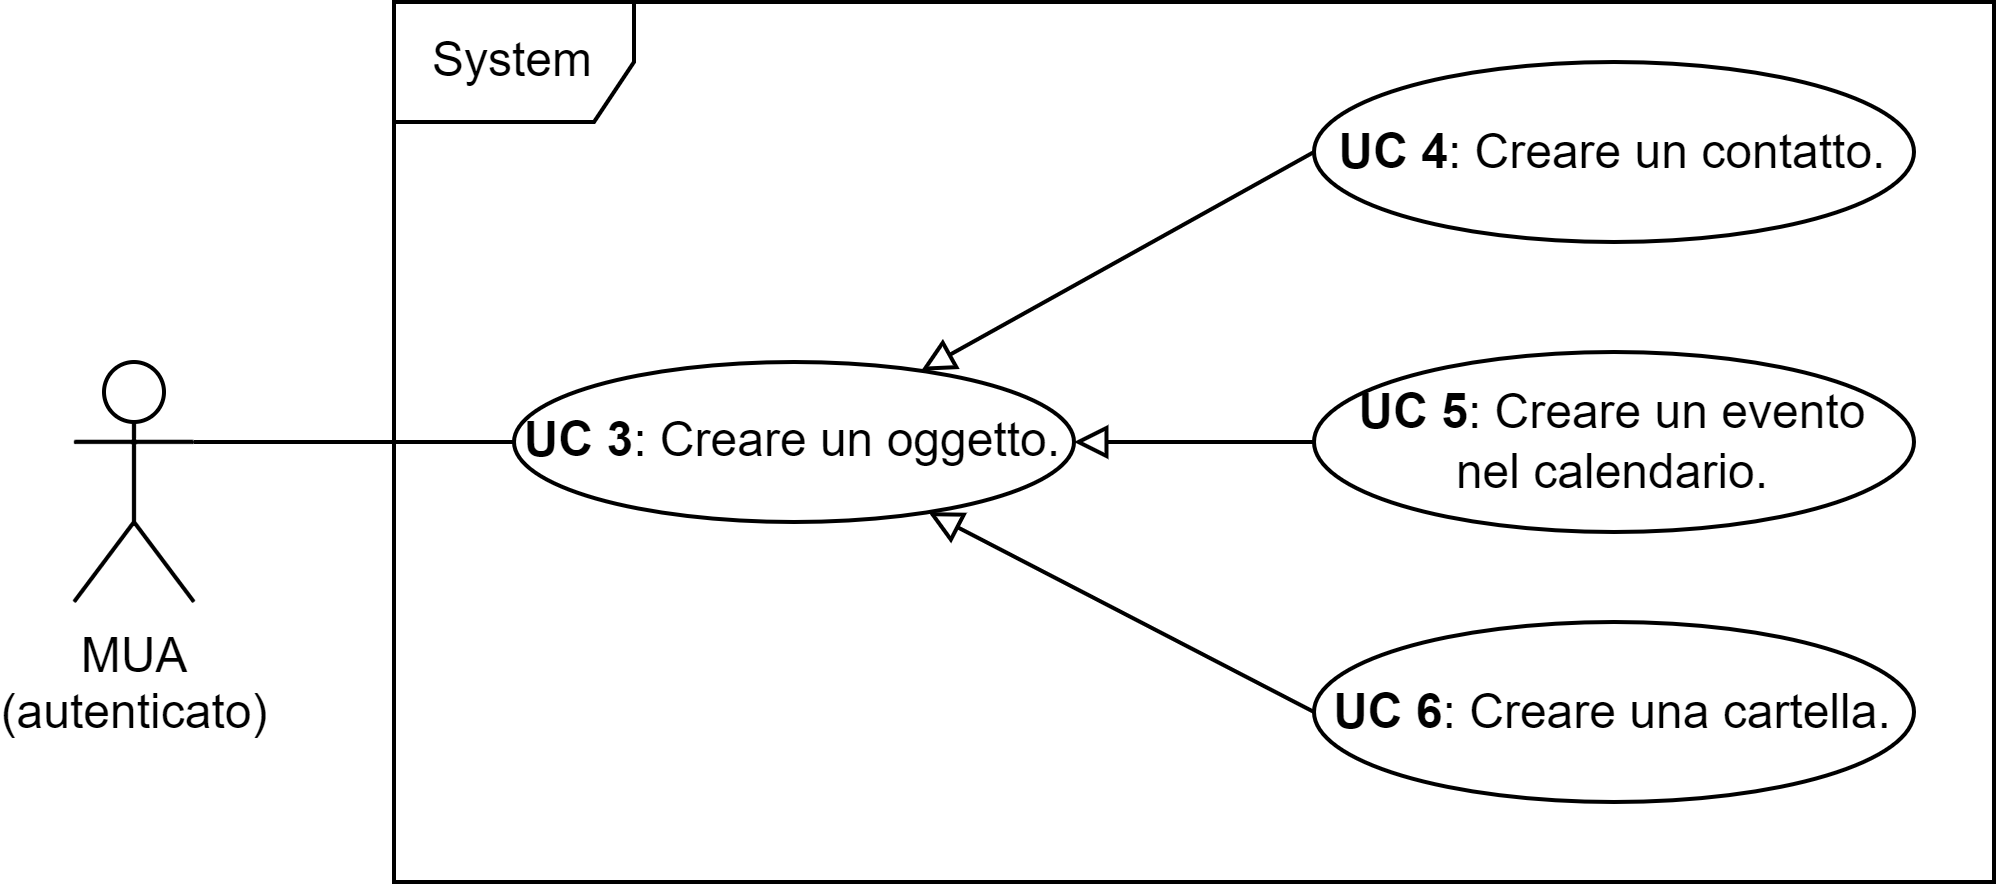
\includegraphics[width=0.85\textwidth]{sections/uc_imgs/UC03.png}
    \centering
    \caption{Diagramma sotto-casi UC 3}
\end{figure}

\subsubsection{UC 3.1 - Trasmette nome cartella} \label{sec:UC3.1}
    \begin{itemize}
        \item \textbf{Attore principale}: MUA;
        \item \textbf{Descrizione}: il MUA trasmette il nome per creare la cartella al sistema;
        \item \textbf{Precondizioni}: il MUA sta usando la funzionalità di creazione di una cartella;
        \item \textbf{Postcondizioni}: il sistema conosce il nome della cartella;
        \item \textbf{Scenario principale}:
            \begin{enumerate}
                \item il MUA invia il nome per creare la cartella al sistema;
                \item il sistema controlla che le informazioni ricevute rispettino il seguente requisito minimo:
                \begin{itemize}
                    \item il nome ricevuto non è una stringa vuota.
                \end{itemize}
            \end{enumerate}
        \item \textbf{Inclusioni}: nessuna;
        \item \textbf{Generalizzazioni}: nessuna;
        \item \textbf{Estensioni}:
            \begin{enumerate}[label=\alph*.]
                \item il sistema non riesce a creare la cartella perché il nome fornito non è valido:
                \begin{enumerate}[label=\arabic*.]
                    \item il sistema ritorna un errore al MUA di nome non valido (\hyperref[sec:UC3.3]{UC 3.3}).
                \end{enumerate}
            \end{enumerate}
    \end{itemize}

    \subsubsection{UC 3.2 - Trasmette id cartella genitore} \label{sec:UC3.2}
    \begin{itemize}
        \item \textbf{Attore principale}: MUA;
        \item \textbf{Descrizione}: il MUA trasmette l'id della cartella genitore al sistema;
        \item \textbf{Precondizioni}: il MUA sta usando la funzionalità di creazione di una cartella;
        \item \textbf{Postcondizioni}: il sistema conosce l'id della cartella genitore;
        \item \textbf{Scenario principale}:
            \begin{enumerate}
                \item il MUA invia le informazioni necessarie per creare la cartella;
                \item il sistema elabora le informazioni ricevute, controlla che:
                \begin{itemize}
                    \item la cartella genitore esista.
                \end{itemize}
            \end{enumerate}
        \item \textbf{Inclusioni}: nessuna;
        \item \textbf{Generalizzazioni}: nessuna;
        \item \textbf{Estensioni}:
            \begin{enumerate}[label=\alph*.]
                \item il sistema non riesce a salvare la cartella perché non trova la cartella genitore:
                \begin{enumerate}[label=\arabic*.]
                    \item il sistema ritorna un errore al MUA di cartella genitore non trovata (\hyperref[sec:UC3.4]{UC 3.4});
                    \end{enumerate}
                \item il sistema non riesce a salvare la cartella perché è un duplicato:
                \begin{enumerate}[label=\arabic*.]
                    \item il sistema ritorna un errore al MUA di cartella duplicata (\hyperref[sec:UC3.5]{UC 3.5}).
                \end{enumerate}
                
            \end{enumerate}
    \end{itemize}



    \subsubsection{UC 3.3 - Ritorna errore nome non valido} \label{sec:UC3.3}
    \begin{itemize}
        \item \textbf{Attore principale}: MUA;
        \item \textbf{Descrizione}: il MUA riceve l'errore che il nome della cartella non è valido;
        \item \textbf{Precondizioni}:  il MUA ha trasmesso il nome per creare la cartella al sistema;
        \item \textbf{Postcondizioni}: il sistema non crea la nuova cartella e il MUA viene notificato dell'errore;
        \item \textbf{Scenario principale}:
            \begin{enumerate}
                \item il sistema controlla la sintassi del nome e trova un errore;
                \item il sistema non crea la cartella e notifica il MUA dell'errore.
            \end{enumerate}
        \item \textbf{Inclusioni}: nessuna;
        \item \textbf{Generalizzazioni}: nessuna;
        \item \textbf{Estensioni}: nessuna.
    \end{itemize}

    \subsubsection{UC 3.4 - Ritorna errore cartella genitore non trovata} \label{sec:UC3.4}
    \begin{itemize}
        \item \textbf{Attore principale}: MUA;
        \item \textbf{Descrizione}: il MUA riceve l'errore che la cartella genitore non è stata trovata;
        \item \textbf{Precondizioni}: il MUA ha trasmesso l'id della cartella genitore al sistema;
        \item \textbf{Postcondizioni}: il sistema non crea la nuova cartella e il MUA viene notificato dell'errore;
        \item \textbf{Scenario principale}:
            \begin{enumerate}
                \item il sistema non trova l'di fornito;
                \item il sistema non crea la cartella e notifica il MUA dell'errore.
            \end{enumerate}
        \item \textbf{Inclusioni}: nessuna;
        \item \textbf{Generalizzazioni}: nessuna;
        \item \textbf{Estensioni}: nessuna.
    \end{itemize}

\subsubsection{UC 3.5 - Ritorna errore cartella duplicata} \label{sec:UC3.5}
    \begin{itemize}
        \item \textbf{Attore principale}: MUA;
        \item \textbf{Descrizione}: il MUA riceve l'errore che la cartella è duplicata;
        \item \textbf{Precondizioni}: il MUA ha trasmesso i dettagli per creare la cartella al sistema;
        \item \textbf{Postcondizioni}: il sistema non crea la nuova cartella e il MUA viene notificato dell'errore;
        \item \textbf{Scenario principale}:
            \begin{enumerate}
                \item il sistema nota che la cartella esiste già e annulla l'operazione per la creazione della cartella;
                \item il sistema non crea la cartella e notifica il MUA dell'errore.
            \end{enumerate}
        \item \textbf{Inclusioni}: nessuna;
        \item \textbf{Generalizzazioni}: nessuna;
        \item \textbf{Estensioni}: nessuna.
    \end{itemize}

